\documentclass[conference]{IEEEtran}
\usepackage[margin=1in]{geometry}
\usepackage{cite}
\usepackage{amsmath,amssymb,amsfonts}
\usepackage{algorithmic}
\usepackage{graphicx}
\usepackage{textcomp}
\usepackage{xcolor}
\usepackage{subcaption}
\usepackage{cuted}

\title{A Four Terminal Charge Pump Model Incorporating Device Leakage Effects}
\author{Mark Lipski}

\begin{document}
	\maketitle
	\section{Abstract}
	This paper constructs a steady state model of the continuous conversion ratio charge pump architecture from first principles, incorporating incomplete charge transfer and finite switch resistance. The model is then verified using a pspice model of the circuit, and the limitations of the assumptions are discussed.
	\section{Introduction}
	
	
	\section{Steady State Model}
	The foundational building block of most Switched Capacitor Power Converter (SCPC) architectures is the circuit in Fig. \ref{Fig:SCCell}, where the flying capacitor connects to 4 unique voltage domains. This flying capacitor cell can then be abstracted as the four terminal device seen in Fig. \ref{Fig:SCCell_Abs}. The SC cell can then be used to construct various dc-dc converter configurations, such as the three stage Dickson in Fig. \ref{Fig:Dickson_Block} or the series parallel converter in Fig. \ref{Fig:SeriesP_Block}.
	
	\begin{figure}
		\centering
		\begin{subfigure}{0.45\linewidth}
			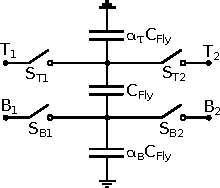
\includegraphics[width=\textwidth]{Figures/SCCell.pdf}
			\caption{Switched capacitor circuit diagram.}
			\label{Fig:SCCell}	
		\end{subfigure}
	\hfill
		\begin{subfigure}{0.45\linewidth}
			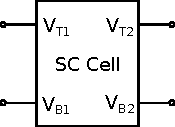
\includegraphics[width=\textwidth]{Figures/SCCell_Abs.pdf}
			\caption{Switched capacitor cell abstraction.}
			\label{Fig:SCCell_Abs}	
		\end{subfigure}
	\caption{Four terminal circuit, and equivalent block level abstraction.}
	\end{figure}
	
	\begin{figure}
		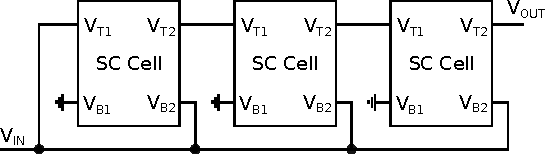
\includegraphics[width=\linewidth]{Figures/Dickson.pdf}
		\caption{Three Stage Dickson configuration using four terminal devices.}
		\label{Fig:Dickson_Block}
	\end{figure}

	\begin{figure}
		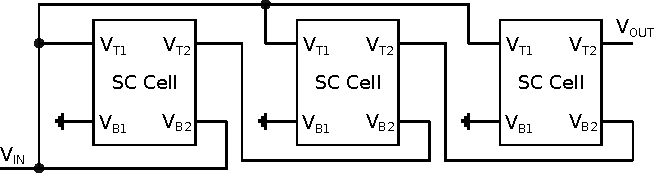
\includegraphics[width=\linewidth]{Figures/SeriesParallel.pdf}
		\caption{Three Stage Series Parallel configuration using four terminal devices.}
		\label{Fig:SeriesP_Block}
	\end{figure}
	
	A steady state circuit representation of the four terminal model can be seen in Fig. \ref{Fig:CircEQ}, where $R_{Fly} = \frac{1}{f_{SW}C_{Fly}}$. However, this model neglects the impact switch resistance has on the equivalent resistance of the cell.
	
	\begin{figure}
		\centering
		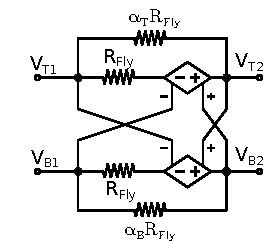
\includegraphics[width=0.6\linewidth]{Figures/CellRes_SSL.pdf}
		\caption{Equivalent circuit model of the four terminal device operating under SSL conditions.}
		\label{Fig:CircEQ}
	\end{figure}
	
	
	The effect of incomplete charge transfer on the output and input charge characteristics of a dc-dc converter has been studied \cite{Tanzawa2011}. However, the model studied assumed ideal clock generation. The following analysis incorporates the resistance of clock drivers into the equations for input and output current. 
	
	\subsection{Incomplete Charge Transfer}
	The associated analysis occurs at steady state with some assumptions:
	
	\begin{figure}
		\begin{subfigure}{0.43\linewidth}
			\centering
			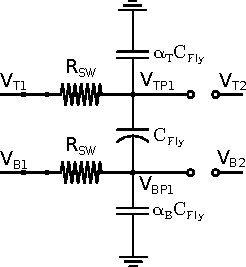
\includegraphics[width=\linewidth]{Figures/Phase1EQ.pdf}
			\caption{Phase 1.}
			\label{Fig:Phase1EQ}
		\end{subfigure}
		\hfill
		\begin{subfigure}{0.43\linewidth}
			\centering
			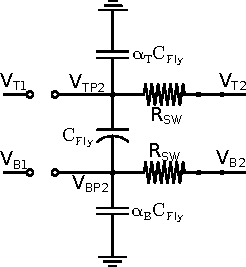
\includegraphics[width=\linewidth]{Figures/Phase2EQ.pdf}
			\caption{Phase 2.}
			\label{Fig:Phase2EQ}
		\end{subfigure}
		\caption{Equivalent representation of \ref{Fig:SCCell}, with switch resistance $R_{SW}$, for both of its phases.}
	\end{figure}
	
	\begin{itemize}
		\item All the capacitors and resistors used in the analysis are linear and time invariant.
		\item The value of $\alpha_T + \alpha_B < 0.1$.
	\end{itemize}
	The circuit in Fig.\ref{Fig:SCCell}, can be represented as Fig. \ref{Fig:Phase1EQ} in its first phase, with Fig. \ref{Fig:Phase2EQ} representing its second phase. The voltage at the top and bottom plates of the capacitor are labeled $V_{TP}$ and $V_{BP}$, $V_{TP1}$ for example, would specify top plate voltage in the first phase.
	
	
	
	
	The first order approximation of $V_{TP1}$ is,
	\begin{equation}
	V_{TP1}(t) = \exp\left(\frac{-t}{\tau}\right)V_{TP1}^{i} + \left(1 - \exp\left(\frac{-t}{\tau}\right)\right)V_{T1},
	\end{equation}
	where $\tau$ is the first order time constant of the circuit, and $V_{TP1}^i$ is the initial value of $V_{TP1}$ at the start of the first phase. 
	
	In order to acquire the value of $\tau$, a frequency domain analysis of the structure in Fig. \ref{Fig:Phase1EQ} can be performed. To simplify the analysis, the value of $V_{B1} = 0$, and the initial conditions on the capacitors are ignored, and the structure is analyzed with respect to $V_{T1}$, the resulting nodal equation at $V_{TP1}$ is 
	\begin{equation}
	\tfrac{V_{TP1} - V_{T1}}{R_{SW}} + s\alpha_T CV_{TP1} + sC(V_{TP1} - V_{BP1}) = 0,
	\end{equation}
	similarly, a nodal analysis at $V_{BP1}$ yields,
	\begin{equation}
	\tfrac{V_{BP1}}{R_{SW}} + s\alpha_B CV_{BP1} + sC(V_{BP1} - V_{TP1}) = 0.
	\end{equation}
	These two nodal equations can then be used to solve for the dominant pole of the circuit, yielding
	\begin{equation}
	V_{TP1} = \tfrac{V_{T1}(sC(\alpha_B + 1))}{s^2C^2R^2(\alpha_B + \alpha_T + \alpha_B\alpha_T) + sRC(2+\alpha_B+\alpha_T) + 1},
	\end{equation}
	however, if it is assumed that $\alpha_T = \alpha_B$ then the simplified expression is,
	\begin{equation}
	V_{TP1} = \tfrac{V_{T1}(sC(\alpha_B + 1))}{(s\alpha_B CR + 1)(sCR(2+\alpha_B) + 1)}.
	\end{equation}
	The resulting first order time constant is then,
	\begin{equation}
	\tau = R_{ON}C_{Fly}\left(2+\alpha_B\right),
	\end{equation}
	The final value of $V_{TP1}$ can be evaluated at $t = \frac{T_{SW}}{2}$, as phase 1 occupies approximately half the period,
	\begin{equation}
	V_{TP1}^f = \exp\left\!(\tfrac{-T_{SW}}{2\tau}\right)V_{TP1}^{i} + \left(1 - \! \exp\!\left(\tfrac{-T_{SW}}{2\tau}\right)\right)V_{T1}.
	\end{equation}	
	Finally, a substitution can be made, relating to the exponential decay at the end of the time step,
	\begin{equation}
	A = \exp\left(-\tfrac{T_{SW}}{2\tau}\right) = \exp\left(\tfrac{T_{SW}}{2R_{ON}C_{Fly}\left(2+\alpha_B\right)}\right),
	\end{equation}
	which can be used to create a simplified expression for $V_{TP1}^f$,
	\begin{equation}
	V_{TP1}^f = AV_{TP1}^i + (1-A)V_{T1}.
	\end{equation}
	A similar procedure can then be repeated for the other nodal voltages,
	\begin{equation}
	V_{BP1}^f = AV_{TP1}^i + (1-A)V_{B1},
	\end{equation}
	\begin{equation}
	V_{TP2}^f = AV_{TP2}^i + (1-A)V_{T2},
	\end{equation}
	\begin{equation}
	V_{BP2}^f = AV_{BP2}^i + (1-A)V_{B2}.
	\end{equation}
	
	The initial conditions of $C_{Fly}$ at the start of each phase can be acquired using the voltage stored on the capacitor. The voltage stored on the capacitor at the end of any phase is $V_{TPx} - V_{BPx}$, where $x$ is the phase. Using the voltage on the capacitor, the initial conditions can be constructed, 
	\begin{equation}
	V_{TP1}^i = \tfrac{V_{TP2}^f - V_{BP2}^f + V_{T1} + V_{B1}}{2},
	\end{equation}
	\begin{equation}
	V_{BP1}^i = \tfrac{V_{BP2}^f - V_{TP2}^f + V_{B1} + V_{T1}}{2},
	\end{equation}
	\begin{equation}
	V_{TP2}^i = \tfrac{V_{TP1}^f - V_{BP1}^f + V_{T2} + V_{B2}}{2},
	\end{equation}
	\begin{equation}
	V_{BP2}^i = \tfrac{V_{BP1}^f - V_{TP1}^f + V_{T2} + V_{B2}}{2}.
	\end{equation}
	Using the equations for the initial conditions and the final voltages, the final voltages can be solved,
	\begin{equation}
	V_{TP1}^f = V_{T1} + \Delta V, 
	\end{equation}
	\begin{equation}
	V_{BP1}^f = V_{B1} - \Delta V,
	\end{equation}
	\begin{equation}
	V_{TP2}^f = V_{T2} - \Delta V,
	\end{equation}
	and
	\begin{equation}
	V_{BP2}^f = V_{B2} + \Delta V
	\end{equation}
	where 
	\begin{equation}
	\Delta V = \frac{A(V_{B1} - V_{T1} - V_{B2} + V_{T2})}{2(A+1)}.
	\end{equation}
	This can then be used to generate the circuit model seen in Fig. \ref{Fig:Circ_Res}, which will incorporate the effects of incomplete charge transfer.
	
	\begin{figure}
		\centering
		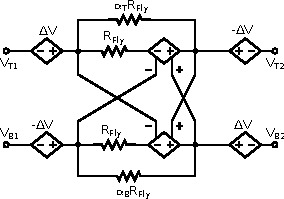
\includegraphics[width=0.7\linewidth]{Figures/CellRes.pdf}
		\caption{Four terminal device model incorporating switch resistance.}
		\label{Fig:Circ_Res}
	\end{figure}

	This can then be verified using simulations of the circuit, in which ideal switches are used. The simulated circuit is the N=3 Dickson Charge pump seen in Fig. \ref{Fig:Dickson_Block}, with two cores per stage 180$^\circ$ out of phase. The parameters used in the circuit are $V_{IN} = 1$V, $V_{OUT} = 3.5$V, C = 1n, $R_{SW}$ = 1$\Omega$. The simulations were run long enough to reach steady state, and the final values were recorded. The output and input currents of the structure were simulated for various frequencies and values of $\alpha_B = \alpha_T$. The corresponding comparisons between the simulation and model data can be seen in Fig. \ref{Fig:Iout_f},  and Fig. \ref{Fig:iin_f}.
	
	\begin{figure}
		\centering
		\includegraphics[width=0.9\linewidth]{Figures/Iout_f.pdf}
		\caption{Comparison of the modelled and simulated output current.}
		\label{Fig:Iout_f}
	\end{figure}

	\begin{figure}
		\centering
		\includegraphics[width=0.9\linewidth]{Figures/Iin_f.pdf}
		\caption{Comparison of the modelled and simulated input current.}
		\label{Fig:iin_f}
	\end{figure}
	
	\subsection{Leakage Effects}
	The leakage effects associated with the transistors are modelled using theory from the \cite{} transistor models. The testing is performed in pspice, using the PTM to simulate the transistors used. 
	
	
		
	\bibliographystyle{IEEEtran}
	\bibliography{leakBib}
	
\end{document}